\documentclass[10pt]{article}
% Report on the two-dimensional point-defect study (11-785). Same layout as midterm_report.tex.
% Every number marked \pd{...} is written by make_report_numbers.py from results/ (pd_numbers.tex).
\usepackage[letterpaper,textwidth=5.5in,textheight=9in,top=1in,headheight=12pt,headsep=25pt,footskip=30pt]{geometry}
\usepackage[T1]{fontenc}
\usepackage[utf8]{inputenc}
\usepackage{mathptmx}
\usepackage{amsmath,amssymb}
\usepackage{microtype}
\usepackage{booktabs}
\usepackage{graphicx}
\usepackage{xcolor}
\usepackage[numbers,sort&compress]{natbib}
\usepackage[small,labelfont=bf]{caption}
\usepackage{enumitem}
\usepackage{tabularx}
\usepackage[colorlinks=true,linkcolor=blue!50!black,citecolor=blue!50!black,urlcolor=blue!50!black]{hyperref}
\setlist{nosep,leftmargin=1.4em}
\setlength{\textfloatsep}{10pt plus 2pt minus 2pt}
\setlength{\floatsep}{8pt plus 2pt minus 2pt}
\renewcommand{\topfraction}{0.92}
\renewcommand{\bottomfraction}{0.6}
\renewcommand{\textfraction}{0.08}
\renewcommand{\floatpagefraction}{0.85}
\setcounter{topnumber}{3}

\newcommand{\repo}{\url{https://github.com/chilalaabubakar/IDL-PROJECT}}
\newcommand{\sig}{\sigma}
\makeatletter
\newcommand{\pd}[1]{\@ifundefined{pd@#1}{\textcolor{red}{[#1]}}{\csname pd@#1\endcsname}}
\newcommand{\pdset}[2]{\expandafter\gdef\csname pd@#1\endcsname{#2}}
\makeatother
\IfFileExists{pd_numbers.tex}{% written by make_report_numbers.py
\pdset{abl-avg-layers1}{17.6}
\pdset{abl-avg-layers2}{13.2}
\pdset{abl-avg-no-weights}{44.3}
\pdset{abl-avg-real-only}{44.5}
\pdset{abl-avg-reference}{44.8}
\pdset{abl-avg-scratch}{13.3}
\pdset{abl-label-layers1-interstitial}{0}
\pdset{abl-label-layers1-vacancy}{0}
\pdset{abl-label-layers2-interstitial}{0}
\pdset{abl-label-layers2-vacancy}{0}
\pdset{abl-label-no-weights-interstitial}{0}
\pdset{abl-label-no-weights-vacancy}{7}
\pdset{abl-label-real-only-interstitial}{17}
\pdset{abl-label-real-only-vacancy}{32}
\pdset{abl-label-reference-interstitial}{18}
\pdset{abl-label-reference-vacancy}{27}
\pdset{abl-label-scratch-interstitial}{0}
\pdset{abl-label-scratch-vacancy}{0}
\pdset{abl-layers1-all}{17.3}
\pdset{abl-layers1-antisite}{15.5}
\pdset{abl-layers1-frenkel}{17.3}
\pdset{abl-layers1-interstitial}{23}
\pdset{abl-layers1-vacancy}{13.5}
\pdset{abl-layers2-all}{23.1}
\pdset{abl-layers2-antisite}{25}
\pdset{abl-layers2-frenkel}{24.7}
\pdset{abl-layers2-interstitial}{27.5}
\pdset{abl-layers2-vacancy}{15.5}
\pdset{abl-no-weights-all}{42.9}
\pdset{abl-no-weights-antisite}{41}
\pdset{abl-no-weights-frenkel}{36.7}
\pdset{abl-no-weights-interstitial}{31.5}
\pdset{abl-no-weights-vacancy}{61}
\pdset{abl-p-layers1}{$p<0.001$}
\pdset{abl-p-layers2}{$p=0.46$}
\pdset{abl-p-no-weights}{$p=0.12$}
\pdset{abl-p-real-only}{$p=0.027$}
\pdset{abl-p-scratch}{$p<0.001$}
\pdset{abl-real-only-all}{42.1}
\pdset{abl-real-only-antisite}{38}
\pdset{abl-real-only-frenkel}{35.3}
\pdset{abl-real-only-interstitial}{29.5}
\pdset{abl-real-only-vacancy}{64}
\pdset{abl-reference-all}{44.7}
\pdset{abl-reference-antisite}{42.5}
\pdset{abl-reference-frenkel}{42}
\pdset{abl-reference-interstitial}{29.5}
\pdset{abl-reference-vacancy}{64}
\pdset{abl-scratch-all}{23.7}
\pdset{abl-scratch-antisite}{26.5}
\pdset{abl-scratch-frenkel}{24}
\pdset{abl-scratch-interstitial}{27.5}
\pdset{abl-scratch-vacancy}{17}
\pdset{abl-updates}{2,000}
\pdset{chance-antisite}{4}
\pdset{chance-frenkel}{5.4}
\pdset{chance-interstitial}{3}
\pdset{chance-max}{5}
\pdset{chance-min}{3}
\pdset{chance-vacancy}{2.9}
\pdset{exp-20k}{50.3}
\pdset{exp-60k}{54}
\pdset{exp-p-cal}{$p<0.001$}
\pdset{exp-p-length}{$p=0.001$}
\pdset{exp-uncal}{50.7}
\pdset{found-best-antisite}{31.5}
\pdset{found-best-frenkel}{32.7}
\pdset{found-best-interstitial}{28}
\pdset{found-best-vacancy}{47.5}
\pdset{found-bonds-antisite}{31.5}
\pdset{found-bonds-frenkel}{27.3}
\pdset{found-bonds-interstitial}{28}
\pdset{found-bonds-max}{31.5}
\pdset{found-bonds-min}{27.3}
\pdset{found-bonds-vacancy}{29}
\pdset{found-energy-antisite}{29}
\pdset{found-energy-frenkel}{32.7}
\pdset{found-energy-interstitial}{28}
\pdset{found-energy-max}{32.7}
\pdset{found-energy-min}{28}
\pdset{found-energy-vacancy}{29.5}
\pdset{found-finder-antisite}{49}
\pdset{found-finder-frenkel}{45.3}
\pdset{found-finder-interstitial}{50}
\pdset{found-finder-vacancy}{69.5}
\pdset{found-geometry-antisite}{16.5}
\pdset{found-geometry-frenkel}{26.7}
\pdset{found-geometry-interstitial}{15}
\pdset{found-geometry-max}{47.5}
\pdset{found-geometry-min}{15}
\pdset{found-geometry-vacancy}{47.5}
\pdset{frenkel-exact-energy}{7}
\pdset{frenkel-exact-finder}{21}
\pdset{gap-finder-energy-max}{40}
\pdset{gap-finder-energy-min}{20}
\pdset{glass-auc}{0.75}
\pdset{glass-clean-cal}{2}
\pdset{glass-clean-raw}{68}
\pdset{glass-def-cal}{28.7}
\pdset{lead-found-antisite}{18}
\pdset{lead-found-frenkel}{13}
\pdset{lead-found-interstitial}{22}
\pdset{lead-found-max}{22}
\pdset{lead-found-min}{18}
\pdset{lead-found-vacancy}{22}
\pdset{lead-restored-antisite}{22}
\pdset{lead-restored-frenkel}{5}
\pdset{lead-restored-interstitial}{16}
\pdset{lead-restored-vacancy}{13}
\pdset{n-antisite}{200}
\pdset{n-frenkel}{150}
\pdset{n-interstitial}{200}
\pdset{n-test}{750}
\pdset{n-vacancy}{200}
\pdset{p-found-bonds-antisite}{<0.001}
\pdset{p-found-bonds-frenkel}{<0.001}
\pdset{p-found-bonds-interstitial}{<0.001}
\pdset{p-found-bonds-vacancy}{<0.001}
\pdset{p-found-energy-antisite}{<0.001}
\pdset{p-found-energy-frenkel}{0.014}
\pdset{p-found-energy-interstitial}{<0.001}
\pdset{p-found-energy-vacancy}{<0.001}
\pdset{p-found-geometry-antisite}{<0.001}
\pdset{p-found-geometry-frenkel}{<0.001}
\pdset{p-found-geometry-interstitial}{<0.001}
\pdset{p-found-geometry-vacancy}{<0.001}
\pdset{p-restored-bonds-antisite}{<0.001}
\pdset{p-restored-bonds-frenkel}{<0.001}
\pdset{p-restored-bonds-interstitial}{<0.001}
\pdset{p-restored-bonds-vacancy}{<0.001}
\pdset{p-restored-energy-antisite}{<0.001}
\pdset{p-restored-energy-frenkel}{0.169}
\pdset{p-restored-energy-interstitial}{<0.001}
\pdset{p-restored-energy-vacancy}{<0.001}
\pdset{p-restored-geometry-antisite}{<0.001}
\pdset{p-restored-geometry-frenkel}{<0.001}
\pdset{p-restored-geometry-interstitial}{<0.001}
\pdset{p-restored-geometry-vacancy}{<0.001}
\pdset{p-worst-found}{p<0.001}
\pdset{p-worst-restored}{p<0.001}
\pdset{ratio-finder-energy-max}{2.4}
\pdset{ratio-finder-energy-min}{1.7}
\pdset{repair-overlap-1}{1--40}
\pdset{repair-overlap-10}{50--73}
\pdset{repair-removed-v1}{7--9}
\pdset{repair-removed-v2}{13--16}
\pdset{restored-best-antisite}{8}
\pdset{restored-best-frenkel}{7.3}
\pdset{restored-best-interstitial}{21.5}
\pdset{restored-best-vacancy}{40.5}
\pdset{restored-bonds-antisite}{7.5}
\pdset{restored-bonds-frenkel}{1.3}
\pdset{restored-bonds-interstitial}{21.5}
\pdset{restored-bonds-max}{22}
\pdset{restored-bonds-min}{1.3}
\pdset{restored-bonds-vacancy}{22}
\pdset{restored-ceiling-antisite}{68.5}
\pdset{restored-ceiling-frenkel}{42}
\pdset{restored-ceiling-interstitial}{80}
\pdset{restored-ceiling-max}{80}
\pdset{restored-ceiling-min}{42}
\pdset{restored-ceiling-vacancy}{67}
\pdset{restored-energy-antisite}{8}
\pdset{restored-energy-frenkel}{7.3}
\pdset{restored-energy-interstitial}{21}
\pdset{restored-energy-max}{26}
\pdset{restored-energy-min}{7.3}
\pdset{restored-energy-vacancy}{26}
\pdset{restored-finder-antisite}{30}
\pdset{restored-finder-frenkel}{12.7}
\pdset{restored-finder-interstitial}{38}
\pdset{restored-finder-vacancy}{53.5}
\pdset{restored-geometry-antisite}{1.5}
\pdset{restored-geometry-frenkel}{0}
\pdset{restored-geometry-interstitial}{8.5}
\pdset{restored-geometry-max}{40.5}
\pdset{restored-geometry-min}{0}
\pdset{restored-geometry-vacancy}{40.5}
\pdset{vacancy-closed}{40}
\pdset{vacancy-open}{60}
}{}% numbers pending: shown in red

\title{Finding and Repairing Point Defects in a Model Glass\\ with a Denoising Network\\[4pt] \large Report on the two-dimensional study}

\author{
  Stacy Cheruto \quad Nicholaus Ladislaus \quad Abubakar Chilala\\ Gentille Uwera \quad Michel Sangwa \quad Boniface Godwin$^{\dagger}$\\[2pt]
  College of Engineering, Carnegie Mellon University Africa\\
  {\small\texttt{\{ccheruto, eladisla, achilala, guwera, sbmichel, bgodwin\}@andrew.cmu.edu}}\\
  {\small $^{\dagger}$Teaching assistant supervising this project}
}
\date{}

\begin{document}
\maketitle

\begin{abstract}
In a crystal, a missing, extra or misplaced atom is found by comparing the structure with its lattice. A glass has no lattice, and once the glass relaxes around such a defect, little of it is left to see. We ask whether a neural network can find the defect from the atom positions alone, and whether the glass can then be returned to the defect-free structure it came from. In a two-dimensional model glass we make the four standard point defects (vacancy, interstitial, Frenkel pair and antisite) by known operations and relax them, so the correct answer is always known. A graph network that starts from a denoising diffusion model of the glass and is then trained to label atoms finds \pd{found-finder-vacancy}\% of vacancies, \pd{found-finder-interstitial}\% of interstitials, \pd{found-finder-antisite}\% of antisites and \pd{found-finder-frenkel}\% of Frenkel pairs. It does not use the interatomic potential. The energy of each atom, which does need the potential, finds \pd{found-energy-min}--\pd{found-energy-max}\%, and the size of each atom's cell, the simplest geometric measure, \pd{found-geometry-min}--\pd{found-geometry-max}\%. Correcting the number or species of atoms at the flagged atom and then minimising the energy restores \pd{restored-finder-vacancy}\%, \pd{restored-finder-interstitial}\%, \pd{restored-finder-antisite}\% and \pd{restored-finder-frenkel}\% of the original glasses. A second network, trained to undo the defect directly, adds nothing once minimisation follows. Finding is what limits the result: when the true location is given, minimisation alone restores \pd{restored-ceiling-min}--\pd{restored-ceiling-max}\%.
\end{abstract}

\section{Introduction}

Point defects are the simplest faults a solid can have. A \emph{vacancy} is a missing atom, an \emph{interstitial} is an extra atom squeezed between the others, a \emph{Frenkel pair} is an atom knocked off its site into a gap (a vacancy and an interstitial together, the basic damage left by irradiation), and an \emph{antisite} is a pair of atoms of different species that have exchanged places~\citep{kittel2005,was2017}. They control diffusion, ageing and the response to radiation. In a crystal each of them is defined against the lattice and can be found by comparing the structure with the ideal sites.

A glass has no lattice~\citep{zachariasen1932}. A point defect can still be \emph{made} in a glass, by removing, adding, moving or swapping an atom, but once the glass relaxes, the neighbours close in and the defect is spread over a few tens of atoms. Early simulations found that most vacancies in a Lennard-Jones glass do not survive relaxation as open holes~\citep{bennett1979}, although some remain and behave like crystal vacancies~\citep{delaye1993}. This makes two questions hard:
\begin{enumerate}
\item \textbf{Find.} Given a relaxed glass that contains one point defect, which atoms are wrong?
\item \textbf{Repair.} What is the defect-free glass it came from?
\end{enumerate}

The usual tools are of two kinds. Geometric measures, such as the free volume around each atom~\citep{starr2002}, need only the positions but are weak, because a glass is full of loosely and tightly packed places that are not defects. Energies and forces are sharper, but they need an interatomic potential, and for many materials no trusted potential exists; structures measured by atomic-resolution microscopy, such as two-dimensional silica glass~\citep{huang2012}, come as positions only. A network that has learned what a normal glass looks like could find what is abnormal from the structure alone. This is where a learned model can add something that a simulation does not already give, and a simulated glass is the right place to test it, because there the defect and the original are known exactly.

This report gives the complete study in a two-dimensional model glass. It replaces the approach of our midterm report, which trained a diffusion model to \emph{place} defects that we had defined ourselves by neighbour counts. After a discussion with Prof.\ Ismaila Dabo we changed the defects to the standard ones, changed the task from placing defects to finding and repairing them, and reduced the method to one network family whose every part has a stated reason (Appendix~\ref{app:feedback}). Our findings are:
\begin{itemize}
\item A learned finder that needs no potential locates three of the four defects \pd{ratio-finder-energy-min}--\pd{ratio-finder-energy-max} times as often as the atom energies do, and more often than cell size for all four (Section~\ref{sec:find}).
\item Once the defect is found, standard energy minimisation does the repair. A network trained to undo the defect learns to move the right atoms, but adds nothing after minimisation and damages the structure without it (Sections~\ref{sec:restore} and~\ref{sec:repairnet}).
\item A quarter of our Frenkel pairs annihilated during relaxation and left no defect. We found this while checking the physics for this report, removed them from the test, and report its consequences openly (Sections~\ref{sec:defects} and~\ref{sec:limits}).
\end{itemize}

\section{Background}

\textbf{Denoising diffusion models of glasses.} Our starting point is DM2~\citep{yang2026dm2}. A network is shown glass structures whose atoms have been shifted by random noise and learns to predict the shifts. Applied repeatedly with decreasing noise, it turns random positions into a realistic glass. Hsu et al.~\citep{hsu2024denoising} used the same idea on crystals for a purpose close to ours: a denoiser removes thermal vibration so that the underlying crystal structure, and its defects, can be identified. Diffusion models have also been used to relax crystals that contain given point defects~\citep{cui2026constrained}. We are not aware of work that finds and repairs point defects in a glass.

\textbf{Learned structural indicators.} Cubuk et al.~\citep{cubuk2015} trained a classifier on local structure to identify the particles of a glass that are about to rearrange. Our finder is similar in spirit, a learned per-atom label from structure alone, but its labels are exact, because we make each defect ourselves.

\textbf{Inherent structures.} Minimising the energy of a configuration takes it to the nearest local minimum of the energy landscape, its inherent structure~\citep{stillinger1982}. A glass has a very large number of such minima. All our glasses, with and without defects, are inherent structures, and ``the same glass'' means the same minimum.

\section{Methods}

\subsection{The glass}

We use the two-dimensional Kob--Andersen mixture~\citep{kob1995,bruning2009}: 65\% large A atoms and 35\% small B atoms that interact through Lennard-Jones pair potentials,
\begin{equation}
u_{\alpha\beta}(r)=4\epsilon_{\alpha\beta}\left[\left(\frac{\sigma_{\alpha\beta}}{r}\right)^{12}-\left(\frac{\sigma_{\alpha\beta}}{r}\right)^{6}\right],
\end{equation}
with $\epsilon_{AA}=1$, $\epsilon_{AB}=1.5$, $\epsilon_{BB}=0.5$, $\sigma_{AA}=1$, $\sigma_{AB}=0.8$ and $\sigma_{BB}=0.88$, cut off and shifted to zero at $2.5\,\sigma_{\alpha\beta}$. Lengths are in units of $\sigma\equiv\sigma_{AA}$ and energies in units of $\epsilon_{AA}$. The strong A--B attraction and the 65:35 composition prevent crystallisation in two dimensions~\citep{bruning2009}. We chose this model because one glass takes seconds to make, so we can afford thousands of defects with exact answers, and because every atom can be drawn and inspected.

Each glass has $N=256$ atoms in a periodic square box of side $14.6\sigma$ (number density 1.2). With LAMMPS~\citep{thompson2022lammps} we melt it at temperature $T=2.0$, cool it to $T=0.01$ at a rate of $10^{-2}$ per time unit, and then minimise its energy. The dataset has 800 training, 100 validation and 100 test glasses. This cooling is fast, so the glasses are poorly annealed, which matters for the antisite (Section~\ref{sec:defects}).

\subsection{The four point defects}
\label{sec:defects}

Each defect is made by a known operation on a defect-free glass (Table~\ref{tab:defects}, Figure~\ref{fig:defects}). The names are used by analogy with crystals: the operations are the same, but a glass has no lattice site that could be empty or doubly occupied and no sublattice for a species to be wrong on, so the defect is defined by the operation that made it. The defected glass is then relaxed: its energy is minimised with every atom free and the box fixed, so it sits in a local minimum as a real defected sample would. Because we know the operation, we know the original glass, which is the exact target for repair, and we need no thresholds to decide what counts as a defect. Each training glass receives 8 defects of each type at random sites (6,400 examples per type); each validation and test glass receives 2 (200 per type). A defect is never made in a glass of another split.

\begin{table}[t]
\centering
\caption{The four point defects and how each is made. The glass is relaxed after the operation.}
\label{tab:defects}
\small
\begin{tabularx}{\linewidth}{@{}l>{\raggedright\arraybackslash}Xc@{}}
\toprule
Defect & Operation on the defect-free glass & Atoms \\
\midrule
Vacancy & remove one atom (A or B, chosen at random) & 255 \\
Interstitial & add one small B atom at the most open point within $2\sigma$ of a random position & 257 \\
Frenkel pair & move one atom to the most open point between $1.2\sigma$ and $3\sigma$ from its site & 256 \\
Antisite & exchange the species of an A atom and its nearest B atom & 256 \\
\bottomrule
\end{tabularx}
\end{table}

\begin{figure}[t]
\centering
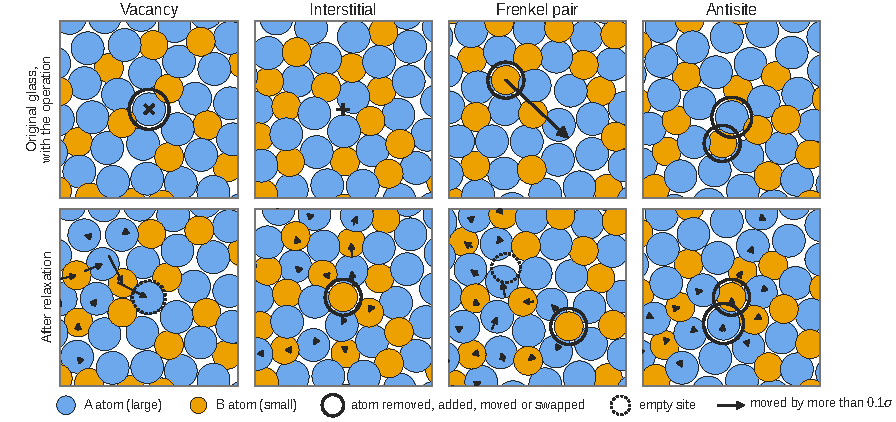
\includegraphics[width=\linewidth]{figures/pd_fig1_defects.pdf}
\caption{The four point defects in test glasses. Top: the original glass and the operation ($\times$ atom removed, $+$ atom added, arrow: atom moved, two rings: species exchanged). Bottom: the same region after relaxation. Each example is the one with the median number of displaced atoms for its type. In the vacancy example, neighbours have moved into the empty site.}
\label{fig:defects}
\end{figure}

\textbf{What the defects become.} We measured each relaxed defect on the test glasses (Table~\ref{tab:physics}).

\emph{Vacancies partly close.} Right after an atom is removed, the most open point at its site is $0.87\sigma$ from the nearest atom. After relaxation this falls to $0.74\sigma$ (median). In defect-free glass the same measure around an atom is $0.63\sigma$, and $0.70\sigma$ at the 95th percentile. About \pd{vacancy-open}\% of the relaxed vacancies are more open than that. The other \pd{vacancy-closed}\% have given up their free volume to the surroundings and no longer stand out as a hole (as in the example of Figure~\ref{fig:defects}). This agrees with early simulations of Lennard-Jones glasses~\citep{bennett1979,delaye1993}.

\emph{A quarter of the Frenkel pairs annihilate.} In 50 of the 200 test Frenkel pairs (and 27\% of the training pairs), the moved atom pushed a neighbour of its own species into the empty site and took that neighbour's place. The relaxed glass is then the original glass with two identical atoms exchanged: the same structure with the same energy, and no defect. Recombination of close Frenkel pairs, also by such replacement of one atom by another, is well known from radiation damage in crystals~\citep{was2017}. Our generator only checked whether the moved atom had returned to \emph{its own} site, so it did not catch these cases. We exclude them from the test, which leaves 150 Frenkel pairs; the consequences for training are discussed in Section~\ref{sec:limits}.

\emph{An antisite does not always cost energy.} The Frenkel pair and the antisite keep all atoms, so the energy difference to the original glass is their formation energy. It is positive for 91\% of the Frenkel pairs (median $3.2\,\epsilon_{AA}$) and for 89\% of the antisites (median $2.8\,\epsilon_{AA}$). In the other 11\% the swapped and relaxed glass is \emph{lower} in energy than the original. In a crystal an antisite always costs energy. A quickly cooled glass is not in its lowest state, and exchanging two atoms can help it to a lower one; this is the principle of the swap Monte Carlo method, which equilibrates glasses by such exchanges~\citep{ninarello2017}. The original glass is still the well-defined target for repair, but in these cases it is not the more stable structure.

\begin{table}[t]
\centering
\caption{The relaxed defects on the test glasses (median, with the middle half of the cases in brackets). ``Atoms displaced'' counts other atoms moved by more than $0.1\sigma$.}
\label{tab:physics}
\small
\begin{tabular}{@{}lcccc@{}}
\toprule
 & Vacancy & Interstitial & Frenkel pair & Antisite \\
\midrule
Real defects in the test & 200 & 200 & 150 & 200 \\
Atoms displaced & 14 [3, 43] & 22 [12, 40] & 44 [21, 69] & 29 [15, 55] \\
Largest displacement of another atom ($\sigma$) & 0.33 & 0.32 & 0.64 & 0.42 \\
Energy above the original ($\epsilon_{AA}$) & -- & -- & 3.2 [1.5, 5.0] & 2.8 [1.4, 4.3] \\
\bottomrule
\end{tabular}
\end{table}

\subsection{Which model is used at each stage, and why}

Table~\ref{tab:stages} lists every tool in the study. The learned parts are one network, a graph network with the symmetries of the problem, used in three ways.

\begin{table}[t]
\centering
\caption{The tool used at each stage and the reason for it.}
\label{tab:stages}
\small
\begin{tabularx}{\linewidth}{@{}l>{\raggedright\arraybackslash}p{1.55in}>{\raggedright\arraybackslash}X@{}}
\toprule
Stage & Tool & Why \\
\midrule
Make glasses & molecular dynamics with the Kob--Andersen potential (LAMMPS) & The physical ground truth. \\
Relax defects; final step of repair & energy minimisation (FIRE~\citep{bitzek2006fire}) & Defines a relaxed glass, and decides which minimum a corrected glass falls into. \\
Learn the glass without labels & periodic EGNN, denoising loss & Learns what normal glass looks like from defect-free glasses only (Section~\ref{sec:equations}). \\
Find the defect & the same EGNN with a per-atom classifier & The answer must not change when the glass is shifted, rotated or its atoms renumbered, and must respect the periodic box. \\
Repair without a potential (tested) & the same EGNN, denoising loss with a defect as the perturbation & Tests whether the network can replace minimisation. \\
Baselines for finding & cell size; atom energy & The simplest structural measure, and the standard measure that uses the potential. \\
\bottomrule
\end{tabularx}
\end{table}

\subsection{The network, and what its equations model}
\label{sec:equations}

\textbf{The graph network.} We use an EGNN~\citep{satorras2021egnn} adapted to a periodic box. Each atom $i$ has a feature vector $h_i$, which starts as an embedding of its species. In each of four layers, every atom exchanges messages with its neighbours $j$ within $2.5\sigma$:
\begin{align}
m_{ij} &= \phi_e\big(h_i,\,h_j,\,|r_{ij}|\big), &
h_i &\leftarrow h_i+\phi_h\Big(h_i,\,\textstyle\sum_j m_{ij}\Big), &
d_i &= \sum_{\text{layers}}\sum_j r_{ij}\,\phi_x(m_{ij}),
\end{align}
where $r_{ij}$ is the shortest vector from atom $i$ to atom $j$ across the periodic box and $\phi_e$, $\phi_h$, $\phi_x$ are small neural networks (a normalisation and a smooth cutoff are left out here). The messages depend only on distances and species, so the features $h_i$ do not change when the glass is shifted or rotated. The output $d_i$ is a sum of neighbour vectors with learned weights, so it turns with the glass. This is the form of a pair force, $F_i=\sum_j r_{ij}\,f(|r_{ij}|)$, except that the weight depends on the whole neighbourhood and not on one distance: the network is a learned many-body force field. It has 0.53 million parameters.

\textbf{The denoising loss.} Following DM2, we take a defect-free glass $x_0$, shift every atom by Gaussian noise of size $\sigma_n$, $x=x_0+\sigma_n\varepsilon$, and train the network to predict the shift:
\begin{equation}
\mathcal{L}=\mathbb{E}\,\big\|d_\theta(x,\sigma_n)-(x-x_0)\big\|^2 .
\label{eq:loss}
\end{equation}
The best possible prediction is the average shift over all glasses that could have produced $x$. By Tweedie's formula~\citep{efron2011,vincent2011} this is $d^{*}(x)=-\sigma_n^{2}\,\nabla\log p_{\sigma_n}(x)$, where $p_{\sigma_n}$ is the distribution of noisy glasses. The correction $-d^{*}$ therefore points towards more probable structures. For a system in thermal equilibrium, $\log p=-U/k_BT$ up to a constant, and the gradient of $\log p$ is the physical force divided by $k_BT$. So the loss teaches the network a \emph{restoring force}. Our glasses are not in equilibrium, so we checked this directly: at $\sigma_n=0.05$ the learned correction and the true Kob--Andersen force point the same way (average cosine 0.81), more closely than the straight line back to the original does (0.68).

\textbf{The finder.} The finder is the same network with a classification layer on the final features: for each atom it gives probabilities for five roles, \emph{intact}, \emph{next to an empty site}, \emph{extra atom}, \emph{displaced atom} and \emph{wrong species}. Because the features are unchanged by shifts, rotations and renumbering, so are the labels. It is trained with cross-entropy on the relaxed defected glasses, with the rare roles weighted up (weights 9--32), because more than 98\% of the atoms are intact. Such weights inflate the predicted probabilities of the rare roles. At test time we subtract the logarithm of each weight from the network's outputs, the standard correction~\citep{menon2021}; it needs no retraining.

\textbf{The repair network.} To test repair without a potential, we train the denoiser on one more kind of perturbation. The input is a defected glass with the number and species of atoms already corrected, plus noise, and the target is again the shift to the original glass (equation~\ref{eq:loss} with $x=x_{\text{corrected}}+\sigma_n\varepsilon$). In the second version the atoms that the defect displaced count 11 times as much in the loss, and most examples have little noise.

\textbf{Training.} The denoiser is trained first, on defect-free glasses only (40,000 updates). The finder and the repair network start from its weights. We use AdamW with learning rate $2\times10^{-4}$, batches of 16 glasses and an exponential moving average of the weights (0.999). One batch in five contains defect-free glasses only, so that the networks learn to leave intact glass alone. The repair network was trained for 20,000 updates per version, and the finder for 20,000 updates followed by 40,000 at half the learning rate, after which its validation scores stopped improving. Each run takes between one and two and a half hours on one T4 GPU.

\subsection{How finding and repair are tested}
\label{sec:test}

All tests use the same \pd{n-test} real defects from the 100 test glasses, and every rate is a fraction of all defects of that type.

\textbf{Found.} Each method gives every atom a score and flags the atom with the highest score. The defect is \emph{found} if the flagged atom lies within $1.5\sigma$ of it (of either site, for a Frenkel pair or an antisite); $1.5\sigma$ covers the nearest neighbours. A randomly chosen atom is that close \pd{chance-min}--\pd{chance-max}\% of the time. The methods are:
\begin{itemize}
\item \emph{Learned finder} (no potential): the probability of the role that belongs to the defect.
\item \emph{Cell size} (no potential, no learning): the area of each atom's Voronoi cell, measured against the mean and spread for its species in defect-free glasses. We flag the largest cell for a vacancy, the smallest for an interstitial, the most unusual for a Frenkel pair, and for an antisite a B atom with too large a cell or an A atom with too small a cell.
\item \emph{Atom energy} (needs the potential): each atom's share of the potential energy, measured against its species in the same way. The highest is flagged. Forces cannot be used, because they vanish in a relaxed glass.
\end{itemize}

\textbf{Restored.} The repair has two steps (Figure~\ref{fig:pipeline}). First the number or species of atoms is corrected at the flagged atom: for a vacancy, an atom of the missing species is put at the most open point within $1.5\sigma$; for an interstitial, the flagged atom is removed; for a Frenkel pair, the flagged atom is moved to one of up to eight open points $1$--$3.2\sigma$ away; for an antisite, a neighbouring A--B pair near the flagged atom is exchanged. Where there is a choice (which open point, which pair), each method chooses with its own score, and the energy route tries every option and keeps the one with the lowest energy. Then the energy is minimised with all atoms free. The glass is \emph{restored} if the result is the original glass: every original atom has an atom of its species within $0.05\sigma$, one to one. Identical atoms may have exchanged places, since that does not change the structure.

The type of defect is taken as known in these tests; only its location is not. As a ceiling we also run the repair with the true location given.

\textbf{Uncertainty.} Brackets are 95\% intervals obtained by resampling whole test glasses (10,000 bootstrap samples), because the two defects made in one glass are not independent. Methods are compared on the same defects with McNemar's exact test.

\begin{figure}[t]
\centering
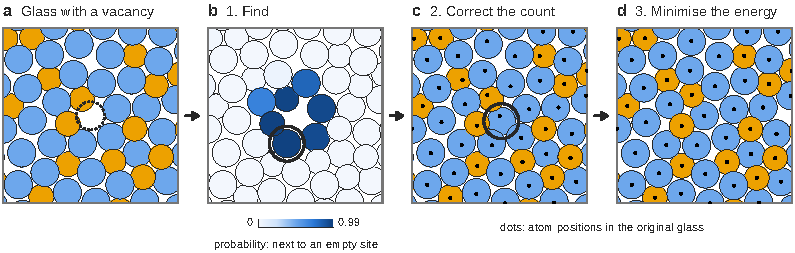
\includegraphics[width=\linewidth]{figures/pd_fig2_pipeline.pdf}
\caption{Finding and repairing one test vacancy. (a)~The relaxed glass; the dotted circle marks where the atom was removed, which the methods are not told. (b)~The finder's probability that each atom is next to an empty site; the flagged atom is ringed. (c)~An atom of the missing species is put at the most open point near the flagged atom. (d)~After energy minimisation every atom sits on its position in the original glass (dots); in (c) the atoms around the defect are still off theirs.}
\label{fig:pipeline}
\end{figure}

\section{Results}

\subsection{Before any training on defects}

The denoiser trained only on defect-free glasses already carries information about defects. Ranking atoms by the size of its predicted correction finds 44\% of vacancies, against 29.5\% for the atom energy. It is poor for interstitials and antisites (12\% and 15\%), and it cannot say which species belongs where. This is the reason for training on defects, and for starting that training from the denoiser.

\subsection{Finding the defect}
\label{sec:find}

\IfFileExists{pd_table_found.tex}{% written by make_report_numbers.py
\begin{table}[t]
\centering
\caption{Defects found (\%): the flagged atom lies within $1.5\sigma$ of the defect. Brackets: 95\% intervals from resampling whole test glasses. Only the atom energy uses the interatomic potential. Bold: the best method.}
\label{tab:found}
\footnotesize\setlength{\tabcolsep}{3.5pt}
\begin{tabular}{@{}lcccccc@{}}
\toprule
 & & \multicolumn{3}{c}{No potential} & Potential & \\
\cmidrule(lr){3-5}\cmidrule(lr){6-6}
Defect & $n$ & Learned finder & Cell size & Unlike neighbours & Atom energy & Random atom \\
\midrule
Vacancy & 200 & \textbf{69.5} {\scriptsize[62, 76]} & 47.5 {\scriptsize[40, 55]} & 29 {\scriptsize[22, 36]} & 29.5 {\scriptsize[23, 36]} & 2.9 \\
Interstitial & 200 & \textbf{50} {\scriptsize[42, 57]} & 15 {\scriptsize[10, 20]} & 28 {\scriptsize[22, 34]} & 28 {\scriptsize[22, 34]} & 3 \\
Antisite & 200 & \textbf{49} {\scriptsize[42, 56]} & 16.5 {\scriptsize[12, 22]} & 31.5 {\scriptsize[25, 38]} & 29 {\scriptsize[23, 35]} & 4 \\
Frenkel pair & 150 & \textbf{45.3} {\scriptsize[38, 53]} & 26.7 {\scriptsize[20, 33]} & 27.3 {\scriptsize[21, 34]} & 32.7 {\scriptsize[25, 40]} & 5.4 \\
\bottomrule
\end{tabular}
\end{table}
}{}

Table~\ref{tab:found} and Figure~\ref{fig:results}a give the main result. The learned finder locates \pd{found-finder-vacancy}\% of vacancies, \pd{found-finder-interstitial}\% of interstitials and \pd{found-finder-antisite}\% of antisites. The atom energy, which needs the potential, finds \pd{found-energy-vacancy}\%, \pd{found-energy-interstitial}\% and \pd{found-energy-antisite}\%, so the finder is ahead by \pd{gap-finder-energy-min}--\pd{gap-finder-energy-max} points (\pd{mcnemar-finder-energy}). Cell size is a serious competitor only for vacancies (\pd{found-geometry-vacancy}\%), where missing volume is what one looks for; even there the finder is \pd{gap-finder-geometry-vacancy} points ahead. For interstitials and antisites, cell size is little better than half of what the energy finds.

Frenkel pairs are the hardest: the finder locates \pd{found-finder-frenkel}\% of the 150 real pairs, against \pd{found-energy-frenkel}\% for the energy and \pd{found-geometry-frenkel}\% for cell size. \pd{frenkel-sentence}

It is worth noting how weak the physical measures are. A relaxed defect has spread its energy and volume over many atoms (Table~\ref{tab:physics}), and a glass has many atoms that are naturally high in energy or loosely packed. The atom with the highest energy is at the defect less than a third of the time.

\begin{figure}[t]
\centering
\IfFileExists{figures/pd_fig3_results.pdf}{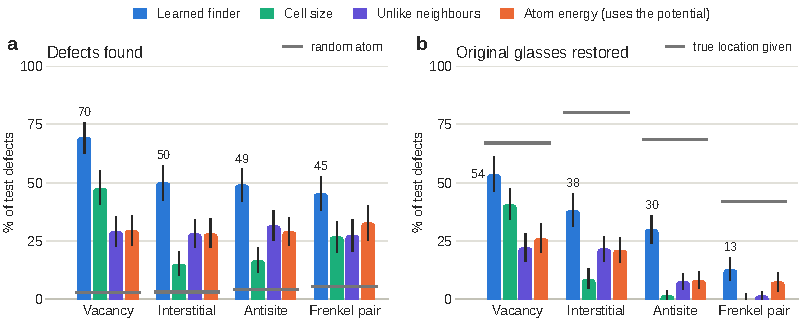
\includegraphics[width=\linewidth]{figures/pd_fig3_results.pdf}}{\fbox{figure pending}}
\caption{(a)~Defects found: the flagged atom is within $1.5\sigma$ of the defect. Grey ticks: a randomly chosen atom. (b)~Original glasses restored after correcting the atoms at the flagged atom and minimising the energy. Grey lines: the same with the true location given. Whiskers: 95\% intervals from resampling test glasses. Numbers above the bars are for the learned finder; all values are in Tables~\ref{tab:found} and~\ref{tab:restored}.}
\label{fig:results}
\end{figure}

\subsection{Restoring the original glass}
\label{sec:restore}

\IfFileExists{pd_table_restored.tex}{% written by make_report_numbers.py
\begin{table}[t]
\centering
\caption{Original glasses restored (\%) after the atoms are corrected at the flagged atom and the energy is minimised (every route uses the potential for this last step). Columns: how the atom was flagged. Last column: the true location given. Brackets as in Table~\ref{tab:found}.}
\label{tab:restored}
\footnotesize\setlength{\tabcolsep}{3.5pt}
\begin{tabular}{@{}lccccc@{}}
\toprule
Defect & Learned finder & Cell size & Unlike neighbours & Atom energy & Location given \\
\midrule
Vacancy & \textbf{53.5} {\scriptsize[46, 61]} & 40.5 {\scriptsize[34, 48]} & 22 {\scriptsize[16, 28]} & 26 {\scriptsize[20, 32]} & 67 {\scriptsize[60, 74]} \\
Interstitial & \textbf{38} {\scriptsize[31, 46]} & 8.5 {\scriptsize[4, 13]} & 21.5 {\scriptsize[16, 27]} & 21 {\scriptsize[16, 26]} & 80 {\scriptsize[74, 86]} \\
Antisite & \textbf{30} {\scriptsize[24, 36]} & 1.5 {\scriptsize[0, 4]} & 7.5 {\scriptsize[4, 11]} & 8 {\scriptsize[4, 12]} & 68.5 {\scriptsize[62, 74]} \\
Frenkel pair & \textbf{12.7} {\scriptsize[8, 18]} & 0 {\scriptsize[0, 2]} & 1.3 {\scriptsize[0, 3]} & 7.3 {\scriptsize[3, 11]} & 42 {\scriptsize[34, 50]} \\
\bottomrule
\end{tabular}
\end{table}
}{}

Table~\ref{tab:restored} and Figure~\ref{fig:results}b show what happens when the correction and the minimisation follow. With the learned finder, \pd{restored-finder-vacancy}\% of vacancy glasses, \pd{restored-finder-interstitial}\% of interstitial glasses and \pd{restored-finder-antisite}\% of antisite glasses return to their original structure, about twice as many as with the atom energy (\pd{restored-energy-vacancy}\%, \pd{restored-energy-interstitial}\% and \pd{restored-energy-antisite}\%). \pd{restored-frenkel-sentence}

Two things stand out. First, restoring follows finding: for each method, the restored rate is roughly three quarters of the found rate for vacancies and interstitials. Second, the ceiling is far above every method. With the true location given, minimisation alone restores \pd{restored-ceiling-vacancy}\% of vacancies, \pd{restored-ceiling-interstitial}\% of interstitials, \pd{restored-ceiling-frenkel}\% of Frenkel pairs and \pd{restored-ceiling-antisite}\% of antisites. What is missing is better finding, not better repair. The ceiling is below 100\% because a glass has many minima close to each other: relaxing the defect moved the neighbours, and putting the atom back does not always lead down to the same minimum the glass started in.

\subsection{The repair network}
\label{sec:repairnet}

We expected the repair network to be the centre of this study. It was not. Its first version learned to remove noise but not the defect, because the defect moves only a few tens of atoms and random noise on all 256 filled the loss. The second version, with the displaced atoms weighted up, did learn the defect: in one step it removes 12--26\% of the error on the displaced atoms, against 6--9\% for the first version.

It still does not help. When minimisation follows, applying the repair network first changes the restored rates by less than their uncertainty (vacancies 51.5\% with it and 51\% without; interstitials 34\% and 34.5\%, measured with the first finder). Once the right atom is added or removed, minimisation finishes the repair by itself. Without minimisation, the network moves the displaced atoms closer to their original positions, sometimes closer than minimisation does, but it pushes atoms onto each other: 20\% of vacancy glasses and half of the Frenkel glasses end with two atoms closer than is ever seen in the data. Applying it repeatedly makes this worse. A network trained only on distances to a target has no notion that atoms cannot overlap, and the interatomic potential supplies exactly that.

\subsection{Is there a defect at all?}

The finder ranks the atoms of a glass that is known to contain a defect. Deciding whether a glass contains one at all is a different question. Without the correction for the class weights, the finder gives some atom a defect probability above one half in \pd{glass-clean-raw}\% of \emph{defect-free} glasses. With the correction this falls to \pd{glass-clean-cal}\%, but then only \pd{glass-def-cal}\% of defected glasses are flagged. Ranking glasses by their highest defect probability separates defected from defect-free ones with an area under the curve of \pd{glass-auc} (0.5 is chance, 1 is perfect). The finder is useful for saying where a defect is, and not yet for saying whether there is one.

\section{Discussion}

\textbf{Why a learned model.} The question from our review was why artificial intelligence should be used at all, when defects can be made without it. Making defects needs no learning, and we no longer do it. Finding them is different. The finder was shown examples of relaxed defects and then locates new ones from positions and species alone, more reliably than either the simplest structural measure or the energies of the potential that made the glass. It can therefore be applied where no potential is available. The simulation's role is to supply examples and to check the answers.

\textbf{What the network adds, physically.} The denoising loss gives the network a model of the forces in normal glass (Section~\ref{sec:equations}), and the finder is built on those features. A relaxed defect is not marked by one atom with too much volume or energy but by a pattern over many atoms (Table~\ref{tab:physics}), and a network that passes messages four times, so that each atom's label depends on the structure up to $10\sigma$ away, can read such a pattern where a single-atom measure cannot.

\textbf{Repair is a job for physics.} Once the right atom is added, removed or exchanged, energy minimisation is fast, exact and free of the overlaps that the repair network produces. We see no reason to replace it when a potential is available. When none is available, a repair network would need at least a built-in rule that atoms cannot overlap.

\subsection{Limits}
\label{sec:limits}

\begin{itemize}
\item \textbf{The Frenkel labels used in training were partly wrong.} 27\% of the training Frenkel pairs had annihilated (Section~\ref{sec:defects}) but were still labelled as defects. The finder was therefore taught to call intact atoms displaced, and its Frenkel result is a lower bound. All test numbers here exclude such cases; the finder has not yet been retrained without them.
\item \textbf{The type of defect is given.} The finder is asked for a vacancy, an interstitial, a Frenkel pair or an antisite. A count of the atoms separates the first two from the others, but not a Frenkel pair from an antisite.
\item \textbf{One defect per glass,} in a small box (256 atoms). Real damage produces many defects that interact.
\item \textbf{A model glass in two dimensions,} at zero temperature. It has no directional bonds and no charges. The defects that matter in a real glass such as silica are of a different kind (broken or extra bonds), which is why we started a study there (Section~\ref{sec:next}).
\item \textbf{``Restored'' is strict.} It asks for the exact original minimum. In a glass, other minima close by are equally natural, and for 11\% of the antisites the defected glass is the more stable one.
\item \textbf{Uncertainty.} With 150--200 defects per type from 100 glasses, the intervals are about $\pm 7$ points wide on each side.
\end{itemize}

\section{Conclusion and next steps}
\label{sec:next}

In a model glass, a graph network that starts from a denoising diffusion model and is trained on relaxed defects finds vacancies, interstitials and antisites without an interatomic potential, more often than the potential's own atom energies and more often than the simplest geometric measure. Correcting the atoms at the flagged site and minimising the energy then restores about twice as many glasses as the energy-based route. A network trained to undo the defect directly is not needed. The room for improvement is in finding: given the true location, minimisation restores \pd{restored-ceiling-min}--\pd{restored-ceiling-max}\% of the glasses.

Next steps, in order:
\begin{enumerate}
\item Retrain the finder without the annihilated Frenkel pairs, and let it name the type of defect.
\item Test the stability of repaired glasses in molecular dynamics, and repeat the study with several defects per glass.
\item Amorphous silica. A first stage without any learned model is complete: with the true site given, minimisation restores 76--96\% of four standard silica defects, but the standard coordination analysis finds only 11--29\% of them. As in two dimensions, finding is the bottleneck, which justifies training a three-dimensional finder.
\end{enumerate}

\section*{Team contributions}
\small
\begin{tabularx}{\linewidth}{@{}l>{\raggedright\arraybackslash}Xl@{}}
\toprule
Workstream & What it covers & Member \\
\midrule
Data and physics & glass generation, potential, relaxation, physical checks of the defects & Nicholaus Ladislaus \\
Defects and evaluation & defect operations, success tests, baselines, statistics & Stacy Cheruto \\
Models and training & EGNN denoiser, finder and repair network; training runs & Abubakar Chilala \\
Repair procedure & correction steps, choice of gap and pair, repair without a potential & Gentille Uwera \\
Baselines and writing & figures, reports & Michel Sangwa \\
Supervision & course teaching assistant; supervised the project & Boniface Godwin \\
\bottomrule
\end{tabularx}
\normalsize

\paragraph{Acknowledgements.} We thank Prof.\ Ismaila Dabo (Materials Science and Engineering, Carnegie Mellon University) for the discussion that redirected this project.

\paragraph{Code and data.} Code, datasets, trained models and every result in this report: \repo{} (branch \path{dabo-point-defects}; the numbers in this report are in \path{results/point_defects_recheck_20261111/}).

\bibliographystyle{abbrvnat}
{\small\bibliography{refs}}

\appendix

\section{How the review shaped this study}
\label{app:feedback}

Prof.\ Dabo raised ten points about the midterm report. Table~\ref{tab:feedback} lists what changed in response.

\begin{table}[h]
\centering
\caption{The points raised in review and the response in this report.}
\label{tab:feedback}
\small
\begin{tabularx}{\linewidth}{@{}r>{\raggedright\arraybackslash}p{1.9in}>{\raggedright\arraybackslash}X@{}}
\toprule
 & Point raised & Response \\
\midrule
1 & Which models are used at each stage, and why? & Table~\ref{tab:stages} states the tool and the reason for every stage. \\
2 & The sections are not connected. & The report follows one question from problem to method, test and result. \\
3 & Methodological and conceptual inconsistencies. & One dataset, one network, one success test and one denominator: every rate is a fraction of all real test defects of a type (Section~\ref{sec:test}). \\
4 & The minimum viable study is in the training section. & The study is that training loss, a network that removes a perturbation from a glass, with a physical defect as the perturbation. \\
5 & What do the equations model? & Section~\ref{sec:equations}: the layer has the form of a force, and the loss teaches a restoring force (cosine 0.81 with the true force). \\
6 & Try reconstructing the original structure from its defected counterpart. & The repair task (Sections~\ref{sec:restore} and~\ref{sec:repairnet}). \\
7 & Or learn to identify incorrect structures. & The finding task, which became the main result (Section~\ref{sec:find}). \\
8 & The defect types follow no concept of computational materials science. & The four standard point defects, made by their defining operations (Table~\ref{tab:defects}), with their relaxed states measured (Table~\ref{tab:physics}). \\
9 & Why use AI to generate defects that can be made without it? & We no longer generate defects. The learned part finds them without a potential, and is compared with two measures that use no learning. \\
10 & The method is too complex. & Removed: defect labels as conditions, guidance, held atoms, the comparison of architectures, hand insertion and the generalisation sweep. \\
\bottomrule
\end{tabularx}
\end{table}

\section{Details}
\label{app:details}

\textbf{Networks.} Periodic EGNN, 4 layers, 128 features per atom, neighbours within $2.5\sigma$, distances expanded in 16 Gaussian functions with a smooth cutoff, 0.53 million parameters. The noise level enters the denoiser and the repair network as 64 Fourier features of $\log\sigma_n$; the finder does not use it. Denoiser: noise $\sigma_n$ between 0.001 and 1. Repair network: $\sigma_n$ between 0.001 and 0.5 (version 1) or log-uniform between 0.001 and 0.3 with the displaced atoms ($>0.1\sigma$) weighted 11 times (version 2). Finder: class weights proportional to (class frequency)$^{-1/2}$, which gives 1, 9.2, 31.7, 31.8 and 22.4 for the five roles.

\textbf{Relaxation.} Defects are relaxed with the FIRE minimiser of LAMMPS to a force tolerance of $10^{-8}$, with the box fixed; a vacancy or an interstitial therefore changes the density by 0.4\%. The repair tests use a FIRE minimiser written in PyTorch (largest force below $10^{-6}$), the same for every method, because it can start from overlapping atoms. The two reach the same minimum from a defect placed in a gap.

\textbf{Open points.} ``The most open point'' is the point of a grid of spacing $0.05\sigma$ that is farthest from every atom, within the stated distance range. \textbf{Cell size in the repair of a Frenkel pair.} The atom with the smallest cell is moved, to the open point whose neighbours have the largest cells.

\textbf{Reproduction.} From the repository root:
\begin{itemize}
\item the test evaluation on real defects (finder, baselines, true location given): \path{scripts/pilots/recheck_real_defects.sh}, which calls \path{scripts/eval_point_defects.py}, \path{scripts/pilots/baseline_routes.py} and \path{scripts/eval_point_defect_repair.py};
\item Table~\ref{tab:physics}: \path{scripts/pilots/point_defect_physics.py};
\item numbers, tables and figures of this report: \path{paper/make_report_numbers.py} and \path{paper/make_report_figures.py}.
\end{itemize}

\end{document}
